% Copyright (C) 2005-2015 Airbus - EDF - IMACS - Phimeca
% Permission is granted to copy, distribute and/or modify this document
% under the terms of the GNU Free Documentation License, Version 1.2
% or any later version published by the Free Software Foundation;
% with no Invariant Sections, no Front-Cover Texts, and no Back-Cover
% Texts.  A copy of the license is included in the section entitled "GNU
% Free Documentation License".
\renewcommand{\filename}{docUC_StocProc_DickeyFuller.tex}
\renewcommand{\filetitle}{UC : Dickey Fuller stationarity tests}

% \HeaderNNIILevel
% \HeaderIILevel
\HeaderIIILevel

\label{DickeyFuller}

\index{Stochastic Process! Dickey Fuller}

This use case details some Dickey Fuller stationarity tests and the strategy proposed by OpenTURNS. The tests are applied on a scalar time series or a sample of scalar time series.

Two forms of non stationarity can be distinguished :
\begin{itemize}
\item deterministic non stationarity when the marginal distribution of the process is time dependent. For example, the mean  is time dependent (temporal trend) or the variance is time dependent;
\item stochastic non stationarity when the random perturbation at time $t$ does not vanish with time (for example a random walk).
\end{itemize}

Specific tests exist to detect the first case. The  Dickey-Fuller tests only focus on the stochastic non stationarity. It assumes that the underlying process, discretized on the time grid $(t_0, \dots, t_{n-1})$  writes :
\begin{equation}\label{DFmodel}
  X_t = a + bt + \rho X_{t-1} + \varepsilon_{t}
\end{equation}
where $\rho > 0$ and where $a$ or $b$ or both $(a,b)$ can be assumed to be equal to 0.

When $(a \neq 0$ and $b=0)$, the model (\ref{DFmodel}) is said to have a \emph{drift}. When $(a = 0$ and $b \neq 0)$, the model (\ref{DFmodel}) is said to have a \emph{linear trend}.

In the  model (\ref{DFmodel}), the only way to have  stochastic non stationarity is to have $\rho = 1$ (if $\rho > 1$, then the time series diverges with time which is readily seen in data). The Dickey-Fuller test in the general case is a unit root test to detect whether $\rho=1$ against $\rho < 1$ :

\begin{equation}\label{DFFormalHypothesis}
  \left\{
  \begin{array}{lr}
    \mathcal{H}_0 : & \rho = 1 \\
    \mathcal{H}_1 : & \rho < 1
  \end{array}
  \right.
\end{equation}

The test statistics and its limit distribution depend on the a priori knowledge we have on $a$ and $b$. In case of absence of a priori knowledge on the structure of the model, several authors have proposed a global strategy to cover all the subcases of the  model (\ref{DFmodel}), depending on the possible values on $a$ and $b$. Figure Fig.\ref{df_strategy} explicitates the strategy  implemented in OpenTURNS,  recommended by Enders (\emph{Applied Econometric Times Series}, Enders, W., second edition, John Wiley \& sons editions, 2004.).



\begin{figure}[H]
  \begin{center}
    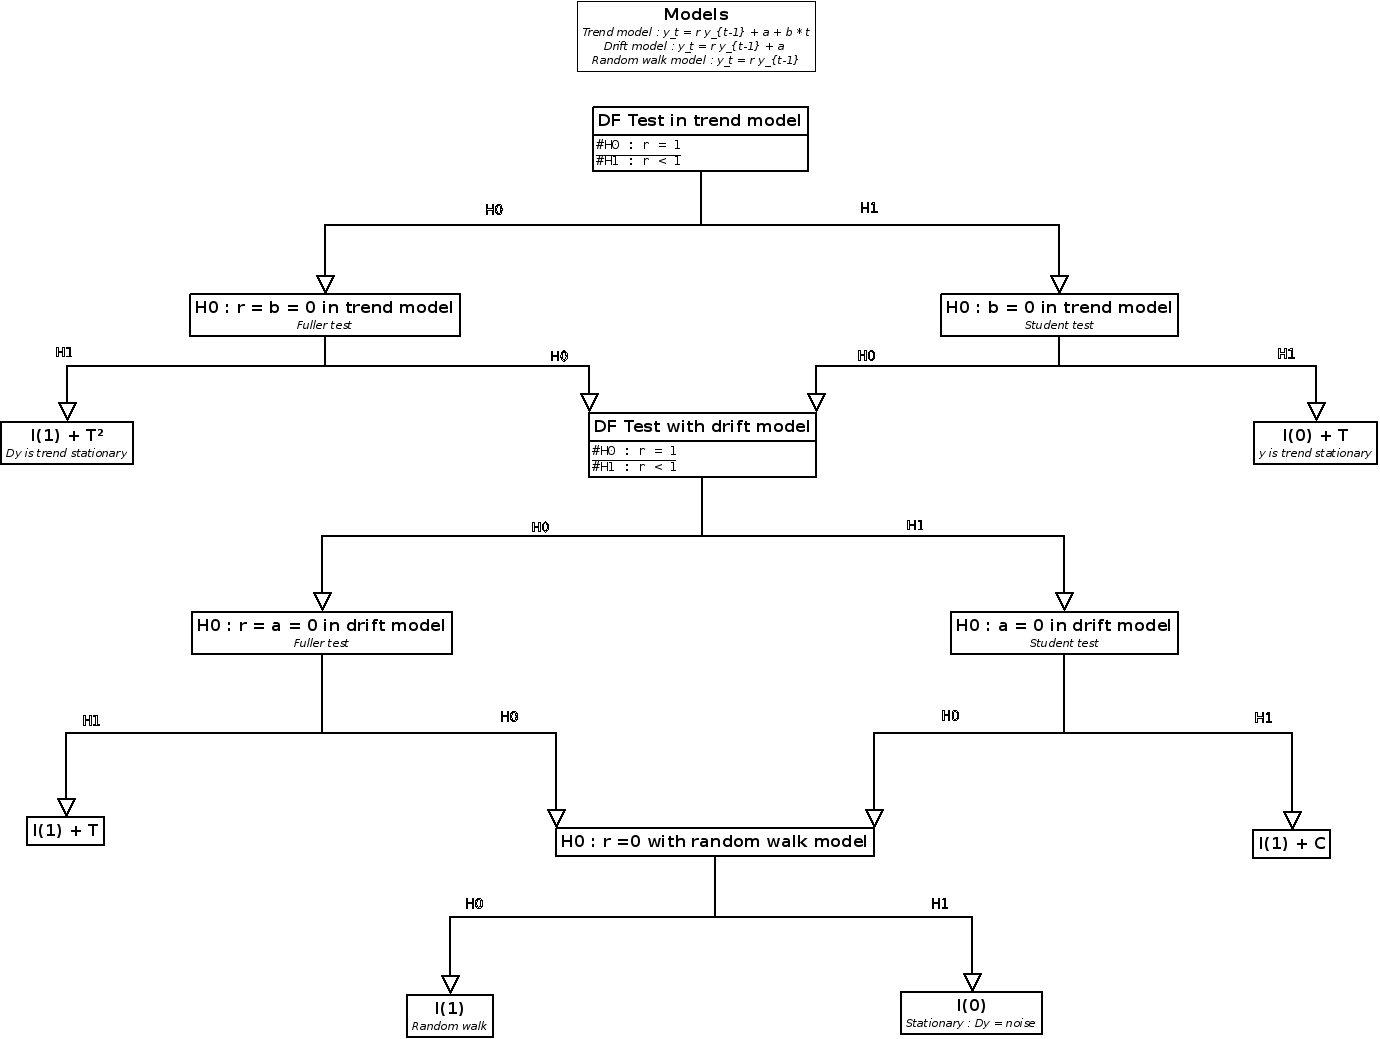
\includegraphics[width=16cm]{Figures/df_strategy.png}
    \caption{Dickey Fuller strategy}
    \label{df_strategy}
  \end{center}
\end{figure}

We note $(X_1, \hdots, X_n)$ the data, by $W(r)$ the Wiener process, and $W^{a}(r) = W(r) - \int_{0}^{1} W(r) dr$, $W^{b}(r) = W^{a}(r) - 12 \left(r - \frac{1}{2} \right) \int_{0}^{1} \left(s - \frac{1}{2} \right) W(s) ds$\\

{\bf We assume the model 1:}
\begin{equation}\label{Model1}
  \boldsymbol{X_t = a + bt + \rho  X_{t-1} + \varepsilon_{t}}
\end{equation}


The coefficients $(a,b,\rho)$ are estimated by $(\Hat{a}_n, \Hat{b}_n, \Hat{\rho}_n)$ using ordinary least-squares fitting, which leads to:
\begin{equation}\label{Model1Estim}
  \underbrace{\left(\begin{array}{lll}
      \displaystyle n-1 &\sum_{i=1}^n t_{i} &\sum_{i=2}^n y_{i-1}\\
      \displaystyle \sum_{i=1}^n t_{i} &\sum_{i=1}^n t_{i}^2 &\sum_{i=2}^n t_{i} y_{i-1}\\
      \displaystyle \sum_{i=2}^n y_{i-1}& \sum_{i=2}^n t_{i}y_{i-1} &\sum_{i=2}^n y_{i-1}^2
    \end{array}
    \right)}_{\mat{M}}
  \left(\begin{array}{c}
    \hat{a}_n\\
    \hat{b}_n\\
    \hat{\rho}_n
  \end{array}
  \right)=
  \left(
  \begin{array}{l}
    \displaystyle \sum_{i=1}^n y_{i} \\
    \displaystyle \sum_{i=1}^n t_{i}  y_{i}\\
    \displaystyle \sum_{i=2}^n y_{i-1} y_{i}
  \end{array}
  \right)
\end{equation}

We first test :
\begin{equation}\label{TestModel1}
  \left\{
  \begin{array}{lr}
    \mathcal{H}_0 :  & \rho = 1 \\
    \mathcal{H}_1 : & \rho < 1
  \end{array}
  \right.
\end{equation}
thanks to the Student statistics :
\begin{equation}\label{stdtStat}
  t_{\rho=1} = \frac{\rho_n-1}{\hat{\sigma}_{\rho_n}}
\end{equation}
where $\sigma_{\rho_n}$ is the least square estimate of the standard deviation of $\Hat{\rho}_n$, given by:
\begin{equation}
  \sigma_{\rho_n}=\mat{M}^{-1}_{33}\sqrt{\frac{1}{n-1}\sum_{i=2}^n\left(y_{i}-(\hat{a}_n+\hat{b}_nt_i+\hat{\rho}_ny_{i-1})\right)^2}
\end{equation}

residual which converges in distribution to the Dickey-Fuller distribution associated to the model with drift and trend:
\begin{equation}
  t_{\rho = 1} \stackrel{\mathcal{L}}{\longrightarrow} \frac{\int_{0}^{1}W^{b}(r) dW(r)}{\int_{1}^{0} W^{b}(r)^2 dr}
\end{equation}
The null hypothesis $\mathcal{H}_0$ from (\ref{TestModel1}) is accepted when $t_{\rho=1} > C_{\alpha}$ where $C_{\alpha}$ is the test threshold of level $\alpha$, which is tabulated in table~\ref{DickeyFullerPval1}.\\

\begin{table}
  \centering
  \begin{tabular}{lccc}
    \hline\noalign{\smallskip}
    $\alpha$ & 0.01 & 0.05 & 0.1 \\
    \noalign{\smallskip}\hline\noalign{\smallskip}
    $C_{\alpha}$ & -3.96 & -3.41 & -3.13 \\
    \noalign{\smallskip}\hline
  \end{tabular}
  \caption{Quantiles of the Dickey-Fuller statistics for the model with drift and linear trend}\label{DickeyFullerPval1}
\end{table}


\begin{itemize}
\item If the null hypothesis  $\mathcal{H}_0$  from (\ref{TestModel1}) is rejected, we test whether $b=0$  :
  \begin{equation}\label{TestSousModele1_1}
    \left\{
    \begin{array}{lr}
      \mathcal{H}_0 :  & b = 0 \\
      \mathcal{H}_1 : & b \neq 0
    \end{array}
    \right.
  \end{equation}
  where the statistics $t_n = \frac{|\hat{b}_n|}{\sigma_{b_n}}$ converges in distribution to the Student distribution $Student(\nu=n-4)$, where $\sigma_{b_n}$ is the least square estimate of the standard deviation of $\Hat{b}_n$, given by:
  \begin{equation}
    \sigma_{b_n}=\mat{M}^{-1}_{22}\sqrt{\frac{1}{n-1}\sum_{i=2}^n\left(y_{i}-(\hat{a}_n+\hat{b}_nt_i+\hat{\rho}_ny_{i-1})\right)^2}
  \end{equation}

  \begin{itemize}
  \item If $\mathcal{H}_0$  from (\ref{TestSousModele1_1}) is rejected, then the model 1 (\ref{Model1}) is confirmed.  And the  test (\ref{TestModel1}) proved that the unit root is rejected : $ \rho < 1$. We then conclude that the final model is : $\boldsymbol{X_t = a + bt +  \rho X_{t-1} + \varepsilon_{t}}$ whith $\boldsymbol{\rho < 1}$ which is a {\bf trend stationary model}.
  \item  If $\mathcal{H}_0$  from (\ref{TestSousModele1_1}) is accepted, then the model 1 (\ref{Model1}) is not confirmed, since the trend presence is rejected and the test (\ref{TestModel1}) is not conclusive (since based on a wrong model). {\bf We then have to test the second model (\ref{Model2})}.
  \end{itemize}


\item If the null hypothesis  $\mathcal{H}_0$  from (\ref{TestModel1}) is accepted, we test
  whether $(\rho, b) = (1,0)$ :
  \begin{equation}\label{TestSousModele1_2}
    \left\{
    \begin{array}{lr}
      \mathcal{H}_0 :  & (\rho, b) =  (1,0) \\
      \mathcal{H}_1 : & (\rho, b) \neq  (1,0)
    \end{array}
    \right.
  \end{equation}
  with the Fisher statistics :
  \begin{equation}\label{stat1}
    \displaystyle \hat{F}_1 = \frac{(S_{1,0} - S_{1,b})/2}{S_{1,b}/(n-3)}
  \end{equation}
  where $S_{1,0}=\sum_{i=2}^n\left(y_i-(\hat{a}_n+y_{i-1})\right)^2$ is the sum of the square errors of the model 1 (\ref{Model1}) assuming $\mathcal{H}_0$ from (\ref{TestSousModele1_2}) and $S_{1,b}=\sum_{i=2}^n\left(y_i-(\hat{a}_n+\hat{b}_nt_i+\hat{\rho}_ny_{i-1})\right)^2$ is the same sum when we make no assumption on $\rho$ and $b$.\\
  The statistics $\hat{F}_1$ converges in distribution to the Fisher-Snedecor distribution $F(2, n-3)$. The null hypothesis $\mathcal{H}_0$  from (\ref{TestModel1}) is accepted when $ \hat{F}_1 < \Phi_{\alpha}$ where $\Phi_{\alpha}$ is the test threshold of level $\alpha$.
  \begin{itemize}
  \item If $\mathcal{H}_0$ from (\ref{TestSousModele1_2}) is rejected, then the model 1 (\ref{Model1}) is confirmed since the presence of linear trend is confirmed.  And the  test (\ref{TestModel1}) proved that the unit root is accepted : $ \rho = 1$. We then conclude that the model is : $\boldsymbol{X_t = a + bt +  X_{t-1} + \varepsilon_{t}}$ which is a {\bf non stationary model}.
  \item  If $\mathcal{H}_0$  from (\ref{TestSousModele1_2}) is accepted, then the model 1 (\ref{Model1}) is not confirmed, since the  presence of the linear trend is rejected and the test (\ref{TestModel1}) is not conclusive (since based on a wrong model). {\bf We then have to test the second model (\ref{Model2})}.
  \end{itemize}

\end{itemize}


{\bf We assume the model 2:}
\begin{equation}\label{Model2}
  \boldsymbol{X_t = a  + \rho  X_{t-1} + \varepsilon_{t}}
\end{equation}

The coefficients $(a,\rho)$ are estimated as follows :
\begin{equation}\label{Model2Estim}
  \underbrace{\left(\begin{array}{lll}
      \displaystyle n-1  &\sum_{i=2}^n y_{i-1}\\
      \displaystyle \sum_{i=2}^n y_{i-1} &\sum_{i=2}^n y_{i-1}^2
    \end{array}
    \right)}_{\mat{N}}
  \left(\begin{array}{c}
    \hat{a}_n\\
    \hat{\rho}_n
  \end{array}
  \right)=
  \left(
  \begin{array}{l}
    \displaystyle \sum_{i=1}^n y_{i} \\
    \displaystyle \sum_{i=2}^n y_{i-1} y_{i}
  \end{array}
  \right)
\end{equation}


We first test :
\begin{equation}\label{TestModel2}
  \left\{
  \begin{array}{lr}
    \mathcal{H}_0 :  & \rho = 1 \\
    \mathcal{H}_1 : & \rho < 1
  \end{array}
  \right.
\end{equation}
thanks to the Student statistics :
\begin{equation}\label{stdtStat}
  t_{\rho=1} = \frac{\rho_n-1}{\sigma_{\rho_n}}
\end{equation}
where $\sigma_{\rho_n}$ is the least square estimate of the standard deviation of $\Hat{\rho}_n$, given by:
\begin{equation}
  \sigma_{\rho_n}=\mat{N}^{-1}_{22}\sqrt{\frac{1}{n-1}\sum_{i=2}^n\left(y_{i}-(\hat{a}_n+\hat{\rho}_ny_{i-1})\right)^2}
\end{equation}
which converges in distribution to the Dickey-Fuller distribution associated to the model with drift and no linear trend:
\begin{equation}
  t_{\rho = 1} \stackrel{\mathcal{L}}{\longrightarrow} \frac{\int_{0}^{1}W^{a}(r) dW(r)}{\int_{1}^{0} W^{a}(r)^2 dr}
\end{equation}
The null hypothesis $\mathcal{H}_0$ from (\ref{TestModel2}) is accepted when $t_{\rho=1} > C_{\alpha}$ where $C_{\alpha}$ is the test threshold of level $\alpha$, which is tabulated in table~\ref{DickeyFullerPval2}.\\

\begin{table}
  \centering
  \begin{tabular}{lccc}
    \hline\noalign{\smallskip}
    $\alpha$ & 0.01 & 0.05 & 0.1 \\
    \noalign{\smallskip}\hline\noalign{\smallskip}
    $C_{\alpha}$ & -3.43 & -2.86 & -2.57 \\
    \noalign{\smallskip}\hline
  \end{tabular}
  \caption{Quantiles of the Dickey-Fuller statistics for the model with drift}\label{DickeyFullerPval2}
\end{table}

\begin{itemize}
\item If the null hypothesis  $\mathcal{H}_0$  from (\ref{TestModel2}) is rejected, we test whether $a=0$  :
  \begin{equation}\label{TestSousModele2_1}
    \left\{
    \begin{array}{lr}
      \mathcal{H}_0 :  & a = 0 \\
      \mathcal{H}_1 : & a \neq 0
    \end{array}
    \right.
  \end{equation}
  where the statistics $t_n = \frac{|\hat{a}_n|}{\sigma_{a_n}}$  converges in distribution to the Student distribution $Student(\nu=n-3)$, where $\sigma_{a_n}$ is the least square estimate of the standard deviation of $\Hat{a}_n$, given by:
  \begin{equation}
    \sigma_{a_n}=\mat{N}^{-1}_{11}\sqrt{\frac{1}{n-1}\sum_{i=2}^n\left(y_{i}-(\hat{a}_n+\hat{\rho}_ny_{i-1})\right)^2}
  \end{equation}

  \begin{itemize}
  \item If $\mathcal{H}_0$  from (\ref{TestSousModele2_1}) is rejected, then the model 2 (\ref{Model2}) is confirmed.  And the  test (\ref{TestModel2}) proved that the unit root is rejected : $ \rho < 1$. We then conclude that the final model is : $\boldsymbol{X_t = a +  \rho X_{t-1} + \varepsilon_{t}}$ whith $\boldsymbol{\rho < 1}$ which is a  {\bf stationary model}.
  \item  If $\mathcal{H}_0$  from (\ref{TestSousModele2_1}) is accepted, then the model 2 (\ref{Model2}) is not confirmed, since the drift presence is rejected and the test (\ref{TestModel1}) is not conclusive (since based on a wrong model). {\bf We then have to test the third  model (\ref{Model3})}.
  \end{itemize}

\item If the null hypothesis  $\mathcal{H}_0$  from (\ref{TestModel2}) is accepted, we test whether $(\rho, a) = (1,0)$ :
  \begin{equation}\label{TestSousModele2_2}
    \left\{
    \begin{array}{lr}
      \mathcal{H}_0 :  & (\rho, a) = (1,0) \\
      \mathcal{H}_1 : & (\rho, a) \neq (1,0)
    \end{array}
    \right.
  \end{equation}
  with a Fisher test. The statistics is :
  \begin{equation}\label{stat1}
    \displaystyle \hat{F}_2 = \frac{(SCR_{2,c} - SCR_{2})/2}{SCR_{2}/(n-2)}
  \end{equation}
  where $SCR_{2,c}$ is the sum of the square errors of the model 2(\ref{Model2}) assuming $\mathcal{H}_0$ from (\ref{TestSousModele2_2}) and $SCR_{2}$ is the same sum when we make no assumption on $\rho$ and $a$.\\
  The statistics $\hat{F}_2$ converges in distribution to the Fisher distribution $F(2, n - 2)$. The null hypothesis $\mathcal{H}_0$  from (\ref{TestModel1}) is accepted if when $ \hat{F}_2 < \Phi_{\alpha}$ where $\Phi_{\alpha}$ is the test threshold of level $\alpha$.
  \begin{itemize}
  \item If $\mathcal{H}_0$  from (\ref{TestSousModele2_2}) is rejected, then the model 2 (\ref{Model2}) is confirmed since the presence of the drift is confirmed.  And the  test (\ref{TestModel2}) proved that the unit root is accepted : $ \rho =1$. We then conclude that the model is : $\boldsymbol{X_t = a  +  X_{t-1} + \varepsilon_{t}}$ which is a {\bf non stationary model}.
  \item  If $\mathcal{H}_0$  from (\ref{TestSousModele2_2}) is accepted, then the model 2 (\ref{Model2}) is not confirmed, since the drift presence is rejected and the test (\ref{TestModel2}) is not conclusive (since based on a wrong model). {\bf We then have to test the third model (\ref{Model3})}.
  \end{itemize}

\end{itemize}


{\bf We assume the model 3:}: \\

\begin{equation}\label{Model3}
  \boldsymbol{X_t = \rho  X_{t-1} + \varepsilon_{t}}
\end{equation}

The coefficients $\rho$ are estimated as follows :
\begin{equation}\label{Model3Estim}
  \hat{\rho}_n=\frac{\sum_{i=2}^ny_{i-1}y_i}{\sum_{i=2}^ny_{i-1}^2}
\end{equation}


We first test :
\begin{equation}\label{TestModel3}
  \left\{
  \begin{array}{lr}
    \mathcal{H}_0 :  & \rho = 1 \\
    \mathcal{H}_1 : & \rho < 1
  \end{array}
  \right.
\end{equation}
thanks to the Student statistics :
\begin{equation}\label{stdtStat}
  t_{\rho=1} = \frac{\hat{\rho}_n-1}{\sigma_{\rho_n}}
\end{equation}
where $\sigma_{\rho_n}$ is the least square estimate of the standard deviation of $\Hat{\rho}_n$, given by:
\begin{equation}
  \sigma_{\rho_n}=\sqrt{\frac{1}{n-1}\sum_{i=2}^n\left(y_{i}-\hat{\rho}_ny_{i-1}\right)^2}/\sqrt{\sum_{i=2}^ny_{i-1}^2}
\end{equation}
which converges in distribution to the Dickey-Fuller distribution associated to the random walk model:
\begin{equation}
  t_{\rho = 1} \stackrel{\mathcal{L}}{\longrightarrow} \frac{\int_{0}^{1}W(r) dW(r)}{\int_{1}^{0} W(r)^2 dr}
\end{equation}
The null hypothesis $\mathcal{H}_0$  from (\ref{TestModel3}) is accepted when $t_{\rho=1} > C_{\alpha}$ where $C_{\alpha}$ is the test threshold of  level  $\alpha$, which is tabulated in table~\ref{DickeyFullerPval3}.\\

\begin{table}
  \centering
  \begin{tabular}{lccc}
    \hline\noalign{\smallskip}
    $\alpha$ & 0.01 & 0.05 & 0.1 \\
    \noalign{\smallskip}\hline\noalign{\smallskip}
    $C_{\alpha}$ & -2.57 & -1.94 & -1.62 \\
    \noalign{\smallskip}\hline
  \end{tabular}
  \caption{Quantiles of the Dickey-Fuller statistics for the random walk model}\label{DickeyFullerPval3}
\end{table}


\begin{itemize}
\item If $\mathcal{H}_0$  from (\ref{TestModel3}) is rejected, we then conclude that the model is : $\boldsymbol{X_t = \rho X_{t-1} + \varepsilon_{t}}$ where $\rho < 1$ which is a {\bf  stationary model}.
\item  If $\mathcal{H}_0$  from (\ref{TestModel3}) is accepted, we then conclude that the model is : $\boldsymbol{X_t = X_{t-1} + \varepsilon_{t}}$ which is a {\bf non stationary model}.
\end{itemize}







OpenTURNS implements the estimation of the coefficients of the different models by the following methods of the object \emph{DickeyFuller}:
\begin{itemize}
\item coefficients of (\ref{Model1Estim}): method \emph{estimateDriftAndLinearTrendModel}
\item coefficients of (\ref{Model2Estim}): method \emph{estimateDriftModel}
\item coefficients of (\ref{Model3Estim}): method \emph{estimateAR1Model}
\end{itemize}


The global DickeyFuller strategy  is implemented in the method \emph{testUnitRoot} of the object \emph{DickeyFuller}. For more expert Users, the different tests of the Dickey-Fuller strategy are implemented by the following methods of the object \emph{DickeyFuller}:
\begin{itemize}
\item test (\ref{TestModel1}) : method \emph{testUnitRootInDriftAndLinearTrendModel}
\item test (\ref{TestSousModele1_1}) : method \emph{testNoUnitRootAndNoLinearTrendInDriftAndLinearTrendModel}
\item test (\ref{TestSousModele1_2}) : method \emph{testUnitRootAndNoLinearTrendInDriftAndLinearTrendModel}
\item test (\ref{TestModel2}) : method \emph{testUnitRootInDriftModel}
\item test (\ref{TestSousModele2_1}) : method \emph{testNoUnitRootAndNoDriftInDriftModel}
\item test (\ref{TestSousModele2_2}) : method \emph{testUnitRootAndNoDriftInDriftModel}
\item test (\ref{TestModel3}) : method \emph{testUnitRootInAR1Model}
\end{itemize}


\requirements
    {
      \begin{description}
      \item[$\bullet$] a time series : {\itshape myTimeSeries}
      \item[type:]  TimeSeries
      \end{description}

      \begin{description}
      \item[$\bullet$] the level of the test : {\itshape level}
      \item[type:]  NumericalScalar
      \end{description}
    }
    {
      \begin{description}
      \item[$\bullet$] a test class : {\itshape myDickeyFullerTest}
      \item[type:]  DickeyFullerTest
      \end{description}

      \begin{description}
      \item[$\bullet$] a test result : {\itshape myTestResult}
      \item[type:]  TestResult
      \end{description}
    }

    \textspace\\
    Python script for this Use Case :

    \begin{lstlisting}
      # Initiate a DickeyFullerTest class
      myDickeyFullerTest = DickeyFullerTest(myTimeSeries)

      # H0 : rho = 1
      # Test = True <=> time series non stationary
      # p-value threshold : probability of the H0 reject zone : 1 - 0.95
      # p-value : probability (test variable decision > test variable decision evaluated on the time series)
      # Test = True <=> p-value > p-value threshold

      # Test of the model (1)
      myTestResultNoConstant = myDickeyFullerTest.testLinearTrendModel(level)

      # Test the model (2)
      # The model contains a drift
      myTestResultNoConstant = myDickeyFullerTest.testDriftModel(level)

      # Test of model (3)
      # The test contains a trend
      myTestResultNoConstant = myDickeyFullerTest.testDriftAndLinearTrendModel(level)

      # Run the strategy test
      myTestResultNoConstant = myDickeyFullerTest.runStrategy(level)

    \end{lstlisting}
